\documentclass{article}
\usepackage{tikz}
\usepackage{amsmath}
\usetikzlibrary{angles,quotes}
\usetikzlibrary{decorations.pathmorphing,calc}
\begin{document}
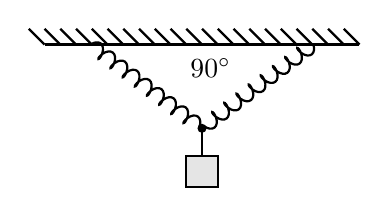
\begin{tikzpicture}[scale=1]
%========================
% Paramètres
%========================
\def\ressortL{2}   % longueur du ressort
\def\masseH{0.4}   % hauteur de la masse
\def\masseL{0.4}     % largeur de la masse
\def\angle{45}     % demi-angle (90° au total)
% ============ AJOUT ============
\def\barreV{0.35}  % longueur de la barre verticale
\def\rayonPt{0.05} % rayon du point (rotule)
% ===============================
% Plafond
%========================
\draw[thick] (-2,0) -- (2,0);
\foreach \x in {-2,-1.8,...,2} {
  \draw[thick] (\x,0) -- (\x-0.2,0.2);
}
%========================
% Points géométriques
%========================
\coordinate (A) at ({-\ressortL*sin(\angle)}, 0);
\coordinate (B) at ({\ressortL*sin(\angle)}, 0);
\coordinate (C) at (0, {-\ressortL*cos(\angle)});
% ============ AJOUT ============
% Point commun d’arrivée des deux ressorts
\coordinate (C) at (0, {-\ressortL*cos(\angle)+\barreV});
% Point d’attache masse / barre
\coordinate (D) at (0, {-\ressortL*cos(\angle)});
% ===============================
% ============ AJOUT ============
% Point commun ressorts / barre
\coordinate (C) at (0, {-\ressortL*cos(\angle)+\barreV});
% Point d’attache barre / masse
\coordinate (D) at (0, {-\ressortL*cos(\angle)});
%========================
% Ressorts obliques
%========================
\node at (0.11,-0.30) {$90^\circ$};
\draw[
  thick,
  decorate,
  decoration={coil, segment length=5.5pt, amplitude=2.5pt}
] (A) -- (C);
\draw[
  thick,
  decorate,
  decoration={coil, segment length=5.5pt, amplitude=2.5pt}
] (B) -- (C);
% Barre verticale
%========================
% ============ AJOUT ============
\draw[thick] (C) -- (D);
% ===============================
% Point (rotule) au point commun
\filldraw[black] (C) circle (\rayonPt);
% Masse suspendue
%========================
\draw[thick, fill=gray!20]
(-\masseL/2, {-\ressortL*cos(\angle)-\masseH})
rectangle
(\masseL/2, {-\ressortL*cos(\angle)});
\end{tikzpicture}
\end{document}